\documentclass[12pt, onecolumn, notitlepage]{scrartcl}
%\documentclass[handout]{beamer}
%\documentclass[draft]{beamer}


\usepackage[utf8]{inputenc}
\usepackage[T1]{fontenc}
\usepackage[english, ngerman]{babel}
\usepackage{graphics} %Für Bilder
\usepackage{graphicx} 
\usepackage{colortbl}
\usepackage{adjustbox}
\usepackage{float}
\usepackage{csquotes}
\usepackage{amssymb}
\usepackage{amsmath}

\restylefloat{table}

\bibliographystyle{ieeetr}

\begin{document}

\renewcommand{\figurename}{Abb.} 


\thispagestyle{empty}
\vspace*{7cm}
\begin{center}
	\Large{
		\textsc{
			Praktikum im großen Studienprojekt \\ [1em]
			\textbf{Verteiltes System zur Berechnung der Mandelbrotmenge} \\ [1em]
			im Wintersemester 2020/21 \\
			bei Prof. Dr. Peter Sturm \\ [1em]
			Universität Trier \\ [1em]
			Lars Klee, 1288210 \\
			Randy Stoppe, 1390338 \\
			Josua Kirsch, 1293138
		}
	}
\end{center}
\setcounter{page}{0}
\newpage

\pagenumbering{roman}
\newpage
	\tableofcontents
\newpage
\pagenumbering{arabic}


\section{Einleitung}
Diese Arbeit entsteht im Rahmen des großen Studienprojektes bei der Professur Systemsoftware und Verteilte Systeme der Universität Trier.
\subsection{Motivation}
\subsection{Problemstellung}
Die Mandelbrotmenge ist die Menge der komplexen Zahlen $c$, für welche die durch die Iteration \begin{align*}
z_{ 0 } &= 0  \\
z_{ n+1 } &= z_{ n }^{ 2 } + c
\end{align*}
definierte Folge $(z_{ n })_{ n\in \mathbb{N} }$ beschränkt ist. Diese lässt sich auf der komplexen Ebene geometrisch interpretieren und bildet ein Fraktal. Wird jedem Punkt auf der komplexen Ebene ein Pixel mit dem entsprechenden Wert von $c$ zugewiesen, ergibt sich eine graphische Darstellung der Mandelbrotmenge. Liegt ein Punkt in der Mandelbrotmenge, so wird ein Pixel schwarz gefärbt, liegt er nicht in ihr, so hängt seine Farbe davon ab, wie schnell die Folge mit dem betreffenden $c$ gegen Unendlich strebt. Diese Berechnung ist äußerst rechenintensiv, jedoch kann jeder einzelne Pixel unabhängig voneinander berechnet werden. Somit bietet sich eine Berechnung der Mandelbrotmenge durch ein verteiltes System an.
\subsection{Zielsetzung}
Das Ziel dieser Arbeit ist es, ein verteiltes System zu entwickeln, das in der Lage ist, die Mandelbrotmenge und dessen Zoomstufen performant zu berechnen. Zu diesem Zweck wird ein Server in Java programmiert, zu dem sich Clients verbinden und Rechenaufträge zur Berechnung der Mandelbrotmenge erhalten können. Der Server selbst rechnet dabei keinen einzigen Punkt der Mandelbrotmenge aus, sondern empfängt die errechneten Ergebnisse der Clients und stellt diese daraufhin graphisch dar. Über die Nutzeroberfläche kann in die Mandelbrotmenge herein- und herausgezoomt werden, wodurch neue Rechenaufträge verteilt werden. \par
Die verschiedenen Clients werden jeweils unter unterschiedlichen Technologien programmiert. So wird der erste Client als Android-Anwendung entwickelt, der zweite Client als CUDA-Anwendung unter Zuhilfenahme des Grafikprozessors und der dritte Client als browserbasierte Anwendung mit JavaScript und WebAssembly. 
\subsection{Gliederung}
Die folgenden drei Kapitel beschreiben jeweils einen der entwickelten Clients und enthalten Unterkapitel, die die zugrundeliegenden Technologien, die Bedienung und letztlich die Entwicklung der Clients und der Probleme, die in dieser auftreten, beschreiben. Zudem werden Vor- und Nachteile der verwendeten Technologoien aufgezeigt.
Daraufhin folgt eine Dokumentation des Servers, die dessen Funktionsweise näher erläutert. Schlussendlich erfolgt eine Reflexion, in der sich damit auseinandergesetzt wird, inwiefern die Zielsetzung erfüllt werden konnte und ob die Verwendung eines verteilten Systems sich als Vorteil für die Berechnung der Mandelbrotmenge erwiesen hat oder nicht.


\section{Android Client}
\subsection{Verwendete Technologie}
Bei der App-Programmierung kann zwischen Kotlin, Java und C++ als Programmiersprachen gewählt werden. Hier wird C++ zur Berechnung der Mandelbrotmenge und Java für die Server-Client-Kommunikation, Button-Listener und zur Überprüfung der WLAN-Verbindung verwendet. Das eigentliche Hauptproblem bei Android oder im Generellen bei Smartphones ist es, dass diese, im Gegensatz zu PCs, beschränkte Ressourcen vorweisen, sei es CPU-Leistung, RAM, Speicherplatz oder Batterielaufzeit. Auch wenn diese Beschränkungen mit neuen Modellen und Technologien immer weiter abnehmen, sollte dennoch dafür gesorgt werden, dass die App möglichst Ressourcen schonend programmiert wird. Außerdem muss bei der App-Programmierung dafür gesorgt werden, dass der main-Thread, auch UI-Thread genannt, möglichst wenig Arbeit auszuführen hat, da dieser, wie der Name bereits andeutet, dafür verantwortlich ist, dass die UI weiterhin auf Eingaben reagieren kann. Wenn dieser Thread zu viel Arbeit verrichten muss, dann kann es nach einer gewissen Zeit zu einer ANR-Meldung (\enquote{Application Not Responding}) kommen. Dann bekommt der Nutzer die Möglichkeit, die App zu beenden oder zu warten, bis die Aufgabe beendet wurde und die UI auf eine Eingabe reagieren kann. Deswegen ist es in der App-Programmierung wichtig, dass der UI-Thread so wenig Instruktionen wie möglich ausführen muss. Dies war zu Beginn des Projekts ein Problem, da diesem immer wieder zu viele Aufgaben zugeteilt worden sind und die App regelmäßig abstürzte. Es sollte sehr viel in neue Threads ausgelagert werden, wie zum Beispiel der Verbindungsaufbau zum Server, aber auch das Verschicken einer einzelnen Nachricht, da sonst die App mit der Fehlermeldung \enquote{NetworkOnMainThreadException} abstürzt.
\subsection{Bedienungsanleitung}
\subsubsection{Starten der Anwendung}
\begin{enumerate}
	\setlength\itemsep{0.07em}
	\item Android Studio starten
	\item Android Projekt (Studienprojekt\_Android) öffnen
	\item Gerät auswählen [Smartphone (a), Emulator (b) oder mehrere Geräte (c)]
	\begin{itemize}
		\item[a)] Smartphone vorbereiten (Entwickleroptionen aktivieren)
		\begin{enumerate}
			\item[1.] Einstellungen öffnen und auf \enquote{Telefoninfo} tippen
			\item[2.] Auf Softwareinformation tippen
			\item[3.] Mehrmals auf Schaltfläche \enquote{Buildnummer} tippen
			\item[4.] Smartphone Pin eingeben
			\item[5.] Nachricht \enquote{Der Entwicklermodus wurde aktiviert} erscheint
			\item[6.] In Einstellungen erscheint Schaltfläche \enquote{Entwickleroptionen}
			\item[7.] Auf Entwickleroptionen tippen
			\item[8.] USB-Debugging aktivieren
			\item[9.] Auf OK tippen
			\item[10.] Smartphone mit USB-Kabel an PC anschließen
			\item[] Entwickleroptionen deaktivieren (nach erfolgreicher Installation der App)
			\begin{itemize}
				\item[1.] Einstellungen öffnen
				\item[2.] Auf Entwickleroptionen tippen
				\item[3.] In erster Zeile auf Regler tippen
			\end{itemize}
		\end{enumerate}
		\item[b)] Wenn Emulator noch nicht erstellt
			\begin{itemize}
			\item[1.] \enquote{AVD Manager} wählen
			\item[2.] \enquote{Create virutal device} wählen
			\item[3.] Beliebiges virtuelles Smartphone wählen
			\item[4.] \enquote{Next} klicken
			\item[5.] Falls vorhanden, aktuellstes Betriebssystem auswählen, ansonsten dieses runterladen und installieren.
			\item[6.] \enquote{Next} klicken
			\item[7.] \enquote{Finish} klicken
			\end{itemize}
		\item[c)] Falls erwünscht, kann mithilfe von \enquote{Run on Multiple Devices} die App auf mehreren Geräten gleichzeitig gestartet werden
			\begin{itemize}
			\item[1.] Auf \enquote{Run on Multiple Devices} klicken
			\item[2.] Alle gewünschten Geräte auswählen
			\item[3.] Auf \enquote{run} klicken (App wird installiert und öffnet automatisch)
			\begin{itemize}
				\item[-] Schritt 4 entfällt somit
			\end{itemize}
		\end{itemize}
	\end{itemize}
	\item App starten (App wird installiert und öffnet automatisch)
\end{enumerate}
\begin{figure}[H] 
	\centering
	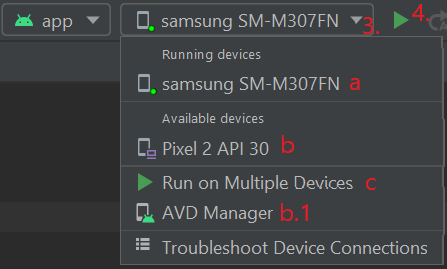
\includegraphics[width=0.6\textwidth]{Geraete_Auswahl_AS.png}
	\caption{zu finden oben in der Mitte von Android Studio}
\end{figure}

Falls beim Öffnen folgender Fehler auftritt:
\begin{figure}[H]
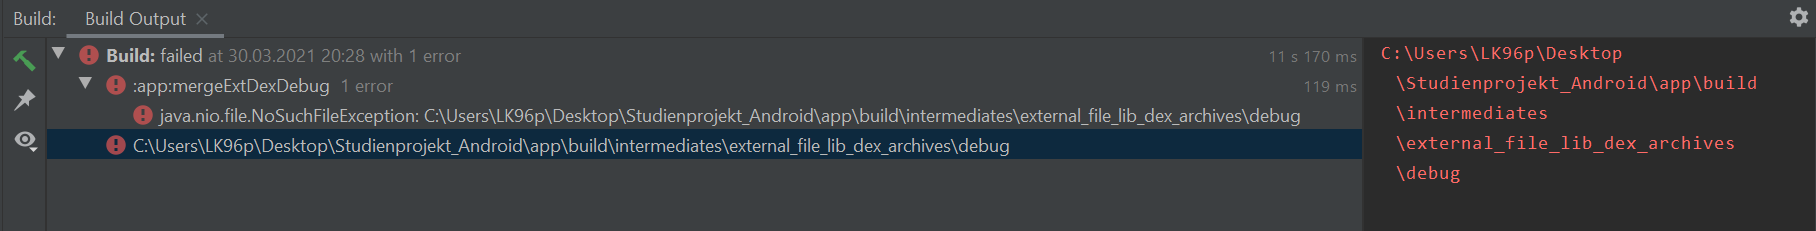
\includegraphics[width=1\textwidth]{build_Fehler.PNG}
\caption{Build failed}
\end{figure}
Dann ist folgendes durchzuführen und anschließend wieder auf App starten zu klicken:
\begin{figure}[H]
\includegraphics[width=1\textwidth]{build_Klick.PNG}
\caption{Fehlerbehebung von Build failed}
\end{figure}
Falls der Fehler \enquote{Invalid Gradle JDK configuration found} auftritt, auf \enquote{Use JDK from project structure} klicken:
\begin{figure}[H]
	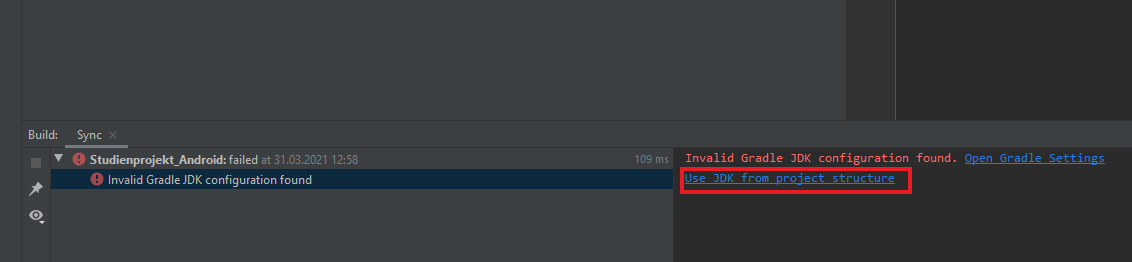
\includegraphics[width=1\textwidth]{invalid_gradle.png}
	\caption{Invalid Gradle JDK configuration found}
\end{figure}

\subsubsection{UI-Erklärung}
Wenn die App gestartet wird und der Startbildschirm (Abb.5) einzusehen ist, dann hat der User die Möglichkeit, am oberen Bildschirmrand einen Namen (Abb.5 a) für das Gerät einzugeben. Dieser wird mit an den Server versendet, da der Androidsocketthread diesen verwendet, um erkennen zu können, welcher Client die Verbindung beendet. Darunter besteht die Möglichkeit, die gewünschte IP-Adresse (Abb.5 b) sowie den Port (Abb.5 c) des Servers einzugeben. Entsprechen die Eingaben den Wünschen, so kann mit einem Tippen auf \enquote{Connect} (Abb.5 d) versucht werden, eine Verbindung zum Server herzustellen. Gelingt dies nicht, so bekommt der User per Toast-Nachricht eine Rückmeldung für die Gründe des gescheiterten Verbindungsversuchs (Server nicht erreichbar, keine WLAN-/Internetverbindung, ungültige/r IP/Port). 
Möchte der User alle Eingaben verwerfen, so besteht diese Möglichkeit, durch ein Tippen auf den Delete-Button (Abb.5 e). \par
Ist eine Verbindung zum Server erfolgreich, so wechselt die Ansicht zum Berechnungsbildschirm (Abb.6). Dort kann der User die CPU-Usage (Abb.6 a) sowie die Memory-Usage (Abb.6 b) einsehen. Zudem kann die Network-Usage (Abb.6 c) eingesehen werden. Diese zeigt an, wie viele kb/s gesendet bzw. empfangen werden. Daraus lässt sich ableiten, ob gerade ein Datenaustausch zwischen Client und Server stattfindet. Oberhalb der Buttons wird der zuvor auf der Startseite eingegebene Gerätename angezeigt (Abb.6 d). Im unteren Drittel des Bildschirms werden die Buttons dargestellt (Abb.6 e). Am unteren Ende des Bildschirms hat der User die Möglichkeit den aktuellen Status, ob eine Berechnung läuft oder pausiert ist, einzusehen (Abb.6 f). Mit einem Tippen auf Start fragt der User den ersten Auftrag an und der Client berechnet daraufhin die Mandelbrotmenge, bis dieser pausiert oder beendet wird. Währenddessen wechselt der Text des Buttons zu \enquote{Running…} (Abb.7). Mit einem Tippen auf Pause wird die aktuell laufende Berechnung beendet und an den Server geschickt, aber kein neuer Auftrag angefordert. Der Pause-Button wechselt währenddessen seine Beschriftung von \enquote{Pause} auf \enquote{Paused} (Abb.8). Wenn die Berechnung wieder aufgenommen werden soll, dann genügt ein antippen des Start-Buttons, der nun die Beschriftung \enquote{Resume} hat. Anschließend wird die Berechnung der Mandelbrotmenge fortgeführt (Abb.9). Durch ein Tippen auf \enquote{Quit} wird die Verbindung zum Server getrennt. Falls eine Berechnung laufen sollte, dann wird der User gefragt, ob er die laufende Berechnung unterbrechen möchte oder nicht (Abb.10). Tippt der User auf \enquote{Quit} und beendet die Berechnung, so wechselt die Ansicht wieder zum Startbildschirm. \\ \\
\underline{\textbf{Anwendungshinweis:}} \par
Es wird nicht empfohlen den Darkmode des Smartphones zur Laufzeit der App zu deaktivieren, da ansonsten eine eventuell laufende Berechnung beendet wird und zwischen Client und Server keine Kommunikation mehr möglich ist.

\begin{figure}[H] 
	\begin{minipage}[b]{.4\linewidth}
		\centering
		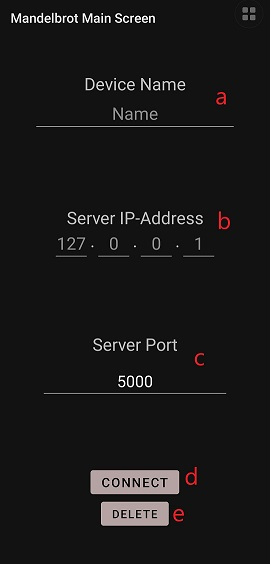
\includegraphics[height=0.5\textheight, width=0.9\textwidth]{start_screen.jpg}
		\caption{Startbildschirm}
	\end{minipage}
	\hspace{.1\linewidth}
	\begin{minipage}[b]{.4\linewidth}
		\centering
		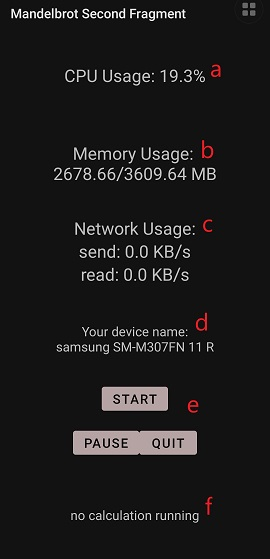
\includegraphics[height=0.5\textheight, width=0.9\textwidth]{calc_screen.jpg}
		\caption{Berechnungsbildschirm}
	\end{minipage}
\end{figure}

\begin{figure}[H] 
	\begin{minipage}[b]{.4\linewidth}
		\centering
		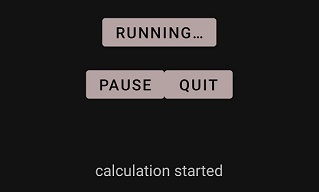
\includegraphics[width=0.8\textwidth]{calc_running.jpg}
		\caption{Berechnung gestartet}
	\end{minipage}
	\hspace{.1\linewidth}
	\begin{minipage}[b]{.4\linewidth}
		\centering
		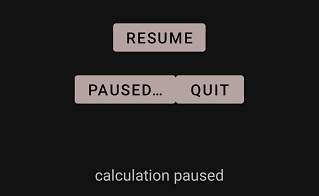
\includegraphics[width=0.8\textwidth]{calc_paused.jpg}
		\caption{Berechnung pausiert}
	\end{minipage}
	\hspace{.1\linewidth}
	\centering
	\begin{minipage}[b]{.4\linewidth}
		\centering
		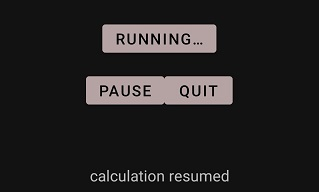
\includegraphics[width=0.8\textwidth]{calc_resumed.jpg}
		\caption{Berechnung fortgesetzt}
	\end{minipage}
\end{figure}

\begin{figure}[H] 
	\centering
	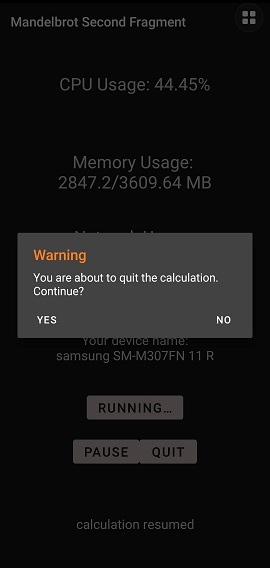
\includegraphics[height=0.5\textheight,width=0.4\textwidth]{calc_quit.jpg}
	\caption{laufende Berechnung beenden}
\end{figure}


\subsection{Entwicklung und Probleme}
Zu Beginn der Entwicklung sollte die App nur den von der App selbst benutzten RAM anzeigen lassen. Dies erwies sich schwieriger als gedacht, denn jede App bekommt vom System eine bestimmte Menge an RAM zur alleinigen Verfügung bereitgestellt. Allerdings benutzen die Apps auch sogenannten \enquote{shared Memory}, den sich mehrere Apps teilen, wodurch die Bestimmung der Menge des benutzten RAMs für eine spezifische App erschwert wird. Aus diesem Grund wird die Gesamtmenge an belegtem RAM angezeigt, um daraus ableiten zu können, ob die App richtig arbeitet. \par
Zwecks Auslesen der CPU-Usage hätte nach ersten Recherchen das Smartphone \enquote{gerootet} werden müssen, da nur dadurch der Zugriff auf die benötigten Informationen möglich ist. Dies ist allerdings nicht zu empfehlen, da das Rooting im schlimmsten Fall zur Unbbrauchbarkeit des Smartphones führt. Zudem können integrierte Sicherheitssysteme nach dem Root-Vorgang nicht mehr aktiviert werden, wodurch das Smartphone anfälliger für Virus- oder Malware-Angriffe ist. Aus diesen Gründen wurde zunächst auf das Rooten und die Anzeige der CPU-Usage verzichtet. Nach weiteren Recherchen wurde eine Lösung, die kein Rooting erfordert, auf den folgenden Internetseiten gefunden:
\begin{itemize}
	\itemsep0pt
	\item http://www.java2s.com/Code/Android/Hardware/GetCPUFrequencyCurrent.htm
	\item http://www.java2s.com/Code/Android/Hardware/GetCPUFrequencyMin.htm
	\item http://www.java2s.com/Code/Android/Hardware/GetCPUFrequencyMax.htm 
\end{itemize}

Aus diesen drei Links wurde dann die gewünschte Lösung abgeleitet (siehe \enquote{CpuInfo.java}).\\
Das Anzeigen der Network-Usage hat von Beginn an zufriedenstellend funktioniert und dient dazu, zu überprüfen, ob eine Kommunikation zwischen Client und Server stattfindet.\\
Nachdem das Anzeigen der Auslastungen umgesetzt wurde und der erfolgreiche Verbindungsaufbau von Client zu Server in einen zusätzlichen Thread ausgelagert worden ist, konnte sich der Berechnung der Mandelbrotmenge und der Versendung der Ergebnisse an den Server gewidmet werden. Die Kommunikation zwischen Client und Server geschieht über TCP. \par
Kommunikation zwischen Client und Server (Version 1.0): 
Der Client hat zur Berechnung alle benötigten Variablen vom Server erhalten (wie genau siehe Dokumentation zu Server-Version 1.0). Anschließend hat der Client durch ein Tippen auf den Start-Button die Berechnung gestartet. In Version 1.0 hat der Client allerdings jedes Pixel des Bildes einzeln an den Server geschickt. Das führte zu einer langen Laufzeit, um nur das Startbild zu berechnen und auf Seiten des Servers darzustellen.\par
Mit dem Wechsel zu Server-Version 2.0 sind diese Probleme behoben, da fortan eine komplette Zeile des Bildes auf der Clientseite berechnet und anschließend an den Server verschickt wird. Dies hat dafür gesorgt, dass die Berechnungsdauer zur Darstellung des Startbilds verkürzt wurde (mehr zur Berechnungsdauer weiter unten). Während des Empfangens der Auftragswerte ergaben sich zunächst Probleme auf Seiten des Clients. Die Aufgaben des Servers wurden als Byte-Array über einen DataOutputStream verschickt, auf Clientseite jedoch mithilfe eines BufferedReaders als String eingelesen, wodurch bei der Kovertierung von String zu Byte-Array Fehler aufgetreten sind. Zum Beispiel wies das empfangene Byte-Array eine falsche Länge auf und der übermittelte Wert konnte nicht aus dem Array rekonstruiert werden. Die Lösung dieses Problems ist es, die nach Erhalt der \enquote{task}-Nachricht empfangenen Pakete, die die relevanten Daten enthalten, um eine Zeile der Mandelbrotmenge zu berechnen, mithilfe eines DataInputStreams einzulesen. Außerdem werden die Werte vom Server nicht mehr als Byte-Array, sondern als int für den x- und itr-Wert bzw. als double für den xMove-, yMove- und zoom-Wert verschickt und auf Clientseite mit readInt() bzw. readDouble() vom DataInputStream eingelesen. Nun kann die Mandelbrotmenge erfolgreich berechnet werden. Allerdings ergaben sich zunächst weitere Probleme, da die Übermittlung der in C++ berechneten Punkte, also einer ganzen Zeile, zu Java nicht richtig funktionierte. Dies wurde zunächst durch Anpassung der initializePackage-Methode in \enquote{Reader.java} behoben. Die Methode wurde in C++ aufgerufen, die jeweiligen x-, y- und itr-Wert jedes for-Schleifendurchlaufs dabei übergeben und daraufhin in \enquote{Reader.java} zu einem String zusammengefasst. Im späteren Verlauf ersetze die format-Methode in C++ die initalizePackage-Methode, woraufhin nur noch einmalig das komplette Paket von C++ an Java übergeben wird. Nachdem ein Paket jetzt erfolgreich erstellt und an den Server versendet wurde, warf der Server eine \enquote{NoSuchElementException}. Diese lag daran, dass die letzten beiden Zeilen eines Paktes wie folgt aussahen: \par
... \par
\enquote{\textbackslash n} \par
\enquote{\textbackslash ntick} \\
Die Exception wurde geworfen als der Server den Zeilenumbruch eingelesen hatte. Dieses Problem konnte gelöst werden, 
indem \enquote{\textbackslash n} entfernt wurde. Solange der Pause-Button nicht angetippt wurde, wird an jedes Paket eine Zeile mit dem Inhalt \enquote{\textbackslash ntask} angefügt. Diese sorgt dafür, dass der Server dem Client einen neuen Auftrag zuschickt. \par
Seitdem kann der Client erfolgreich Aufträge entgegennehmen, diese berechnen und vom Server verwendbare Antworten an den Server zurückschicken. Nun traten allerdings \enquote{StackOverflowExceptions} auf Seiten des Servers auf. Diese entstanden dadurch, dass die sendTask-Methode des Servers nach Verschicken des Iterationswerts erneut die recieveMessage-Methode aufrief, obwohl dieser Aufruf nicht nötig war und somit gelöscht werden konnte. \par
Die Check-Klasse sorgt dafür, dass im Fall einer schwachen Internetverbindung, die Verbindung zum Server getrennt wird oder im Fall eines kompletten Verbindunsabbruchs, die Ansicht auf dem Bildschirm wieder zum Startbildschirm wechselt. Zunächst wechselte die Ansicht nicht zum Startbildschirm zurück, wenn die WLAN-Verbindung unterbrochen wurde, da bei der Überprüfung, welche Ansicht (Fragment) zur Zeit aktiv ist, ein Fehler unterlaufen ist. Mithilfe des \enquote{FragmentManagers} konnte dieses Problem gelöst werden, denn \enquote{fragmentManager.getPrimaryNavigationFragment()} liefert das aktuelle aktive Fragment und somit kann der Befehl \\
\enquote{\textit{NavHostFragment.findNavController(Objects.requireNonNull(fragmentManager\\.getPrimaryNavigationFragment())).navigate(R.id.action\_secondFragment\_to\\\_firstFragment)}} \\
erfolgreich ausgeführt werden. Das gleiche Problem trat zudem beim Tippen auf den Quit-Button auf und konnte auf gleichem Wege gelöst werden. \par
Durch Zufall fiel auf, dass im Logcat, wenn zur zweiten Ansicht gewechselt wird, jede Sekunde zwischen 30 und 40 Frames  übersprungen werden, da der UI-Thread zu viel Arbeit verrichtet. Das liegt vermutlich daran, dass jede Sekunde die CPU-Usage, Memory-Usage sowie die Network-Usage aktualisiert werden und dieser Vorgang muss auf dem UI-Thread laufen, da dieser der einzige ist der die UI aktualisieren kann. Die Benutzeroberfläche reagiert allerdings noch auf jede Eingabe und dies stellt somit kein schwerwiegendes Problem dar und kann ignoriert werden. \par
Ein weiteres Problem besteht darin, dass, nachdem die App beendet, das Smartphone erneut mit dem PC über ein USB-Kabel  verbunden sowie Android Studio neugestartet wurden, weiterhin Ausgaben im Logcat stattfinden. Es können allerdings keine neuen Berechnungen sein, da der Zeitstempel, wie in den beiden folgenden Bildern zu erkennen, identisch ist.

\begin{figure}[htbp] 
	\centering
	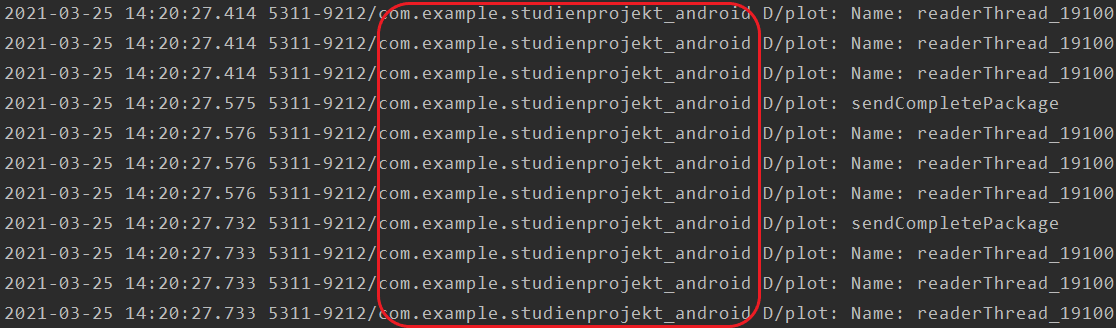
\includegraphics[width=0.8\textwidth]{Logcat_laufend.PNG}
	\caption{Logcatausgabe bei laufender App}
\end{figure}

\begin{figure}[htbp] 
	\centering
	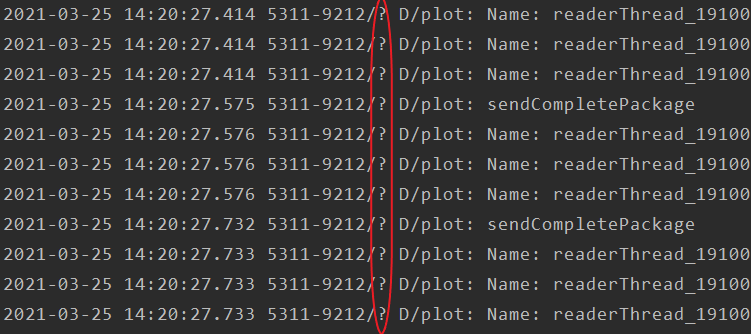
\includegraphics[width=0.8\textwidth]{Logcat_nichtLaufend.PNG}
	\caption{Logcatausgabe bei nicht laufender App}
\end{figure}

Die Ursache dieses Problems kann nicht darin liegen, dass der \enquote{readerThread} bei Beendigung der App nicht richtig terminiert wird, da ein Aufruf von \enquote{readerThread.interrupt()} nicht hilft. Wenn die App deinstalliert und das Smartphone neugestartet wird, dann wird bei Android Studio in Logcat nichts mehr ausgegeben. Deswegen wird empfohlen, wenn die App auf dem eigenen Smartphone ausgeführt wird, nach der Deinstallation das Smartphone neu zu starten. \\ \\
\textbf{Berechnungsdauer (Startbild) via Internet:}
\begin{table}[H] 
	\centering
	\scalebox{0.9}{
		\begin{tabular}{!{\color{black}\vrule}c!{\color{black}\vrule}c!{\color{black}\vrule}} 
			\cline{1-1}\arrayrulecolor{black}\cline{2-2}
			Server-Version
			1.0 & Server-Version
			2.0                                                                                                                                                                         \\ 
			\arrayrulecolor{black}\cline{1-1}\arrayrulecolor{black}\cline{2-2}
			\multicolumn{2}{!{\color{black}\vrule}c!{\color{black}\vrule}}{\begin{tabular}[c]{@{}c@{}}Auflösung:			1260x625 \\Iterations:			50 \\Anzahl			Clients: 1 \\			Client-Typ:			Android \\Messung			1\end{tabular}}       \\ 
			\arrayrulecolor{black}\hline
			ca.
			300 Sekunden   & ca. 210 Sekunden                                                                                                                                                                              \\ 
			\hline
			\multicolumn{2}{!{\color{black}\vrule}c!{\color{black}\vrule}}{\begin{tabular}[c]{@{}c@{}}Auflösung:			500x500 \\Iterations:			50 \\			Anzahl			Clients: 1 \\Client-Typ:\\			Android			Messung			2\end{tabular}}      \\ 
			\hline
			nicht
			gemessen     & ca.
			70 Sekunden                                                                                                                                                                            \\ 
			\hline
			\multicolumn{2}{!{\color{black}\vrule}c!{\color{black}\vrule}}{\begin{tabular}[c]{@{}c@{}}Auflösung:			500x500 \\			Iterations:			200 \\Anzahl			Clients: 1 \\			Client-Typ:			Android \\Messung			3\end{tabular}}    \\ 
			\hline
			nicht
			gemessen     & ca.
			80 Sekunden                                                                                                                                                                            \\ 
			\hline
			\multicolumn{2}{!{\color{black}\vrule}c!{\color{black}\vrule}}{\begin{tabular}[c]{@{}c@{}}Auflösung:			1000x1000 \\Iterations:			200 \\Anzahl			Clients: 1 \\Client-Typ:			Android \\Messung			4\end{tabular}}        \\ 
			\hline
			nicht
			gemessen     & ca.
			165 Sekunden                                                                                                                                                                           \\
			\hline
		\end{tabular}
	}
	
\end{table}

Messungen 2, 3 und 4 konnten bei der Server-Version 1.0 nicht gemessen werden, da die Auflösung nicht angepasst werden konnte. Es ist allerdings gut erkennbar, dass die benötigte Zeit von Server-Version 1.0 zu 2.0 stark reduziert wurde. Des Weiteren ist gut zu erkennen, dass die Erhöhung der Iterationen keinen drastischen Einfluss auf die Berechnungsdauer hat (Messungen 2 und 3), denn die benötigte Zeit hat sich im Gegensatz zur Iteration nicht vervierfacht. Einen viel größeren Einfluss auf die Zeit nimmt hingegen die Größe der Auflösung (Messungen 3 und 4). Hier wurde jeweils die Höhe und Breite verdoppelt, die Fläche entsprechend vervierfacht, die benötigte Zeit hat sich circa verdoppelt.


\section{CUDA Client}
\subsection{Verwendete Technologie}
Compute Unified Device Architecture (CUDA) ist eine im Jahr 2007 von NVIDIA entwickelte Architektur zur parallelen
Berechnung auf hauseigenen Grafikkarten. Diese wird bis heute von allen Grafikprozessoren der Generation G80 und aufwärts unterstützt 
und stetig weiterentwickelt. Mit CUDA verfolgt NVIDIA das Ziel, das Feld der \enquote{general-purpose computing on graphics processing units} (GPGPU) 
voranzutreiben und Softwareentwicklern ohne speziellem Hintergrundwissen in der Grafikkartenprogrammierung zu ermöglichen, die enorme parallele Rechenleistung 
der Grafikkarte für computergrafikberechnungsferne Anwendungen nutzen zu können. \newline
Das Schreiben erster sogenannter CUDA-Kernels gestaltet sich 
für Entwickler mit C/C++ Hingergrund als besonders angenehm, da mit \enquote{CUDA for C/C++} eine sehr mächtige API zur Verfügung steht, die
die bekannte C/C++ Syntax nur um einige wenige Schlüsselwörter ergänzt. \newline 
Erste Kernels lassen sich anhand der umfangreichen Dokumentation von NVIDIA 
schnell umsetzen. Um allerdings wirklich effiziente Programme für Grafikprozessoren zu schreiben, sollte ein grundlegendes Verständnis des Aufbaus der 
\enquote{CUDA-enabled} Grafikprozessoren vorhanden sein und das Management von globalem, geteiltem und konstantem Speicher verstanden werden.\newline
CUDA folgt einer hierarchischen Struktur. Oberste Ebene bildet das sogenannte \enquote{Grid}, das mehrere Threadblöcke zusammenfasst. Ein Threadblock umfasst seit 2019 bis zu 1024 Threads.
Ein beispielhafter Kernelaufruf \newline
\newline
\textit{kernel\_function}$<<<$Anzahl Blöcke, Anzahl Threads pro Block$>>>$(A, B, C) \newline
\newline
legt ein entsprechendes 
\enquote{Grid} mit der entsprechenden Anzahl an entsprechend dimensionierten Threadblöcken an und übergibt die Parameter A, B und C. Die Parameter sind fortan im lokalen Speicher jedes Threads verfügbar.
Da zwischen Host und Device Speicher hin- und hergewechselt werden muss, sollte mindestens einer der übergebenen Parameter ein entsprechender Pointer auf ein zuvor über \enquote{cudaMalloc} alloziiertes Gerätespeichersegment sein, in dem die Ergebnisse der GPU abgelegt werden. 
Dieses Speichersegment wird dann nach Beendigung des Kernels in ein entsprechend großes Speichersegment des Hosts kopiert. Diese Transfers sollten allerdings mit Bedacht durchgeführt werden, da sie äußerst kostspielig sind.\newline
Alle Blöcke eines \enquote{Grids} führen immer denselben Kernel aus. 
Zudem gilt es zu beachten, dass Threadblöcke auf der Hardwareseite von CUDA-fähigen GPUs in sogenannten \enquote{Warps} organisiert sind. Ein \enquote{Warp} ist eine Menge von 32 Threads, die pro Clockzyklus immer dieselbe Instruktion ausführen müssen. Daher gilt es, \enquote{Warp}-Divergenz zu
vermeiden, also Bedingungen im Code, die einen unterschiedlichen Programmablauf innerhalb eines \enquote{Warps} verursachen können. Wenn ein Teil des Warps den einen Pfad gehen muss und der andere Teil einen Anderen, so werden die Instruktionen nicht mehr parallel, sondern sequentiell ausgeführt. \newline
Der Aufbau eines \enquote{CUDA for C/C++} Programms ist nahezu identisch zu einer normalen C/C++-Datei. Das gilt für Header- als auch für Sourcedateien.
Die einzigen Unterschiede sind die Dateiendung (.cu statt .c bzw. .cuh statt .h) und die Verwendung der folgenden Schlüsselwörter
\begin{itemize}
\item \underline{\hspace{0.5cm}}host\underline{\hspace{0.5cm}} (kennzeichent Code, der auf der CPU läuft und nur von dieser aufgerufen werden kann)
\item \underline{\hspace{0.5cm}}global\underline{\hspace{0.5cm}} (kennzeichnet Kernelmethoden, die durch den Host gestartet werden können) 
\item \underline{\hspace{0.5cm}}device\underline{\hspace{0.5cm}} (kennzeichnet Code, der auf der GPU läuft und nur durch Kernel- bzw. andere Devicemethoden aufgerufen werden kann) 
\item \underline{\hspace{0.5cm}}shared\underline{\hspace{0.5cm}}
(markiert Variablen, die in den geteilten Speicher geladen werden sollen) 
\end{itemize}  
Zusätzlich werden Kernelfunktionsaufrufe, wie zuvor bereits gesehen, durch ein \newline
$<<<...>>>$ markiert, in welchem die Launchkonfigurationen (Anzahl der Blöcke, Anzahl der Threads pro Block und optional eine Menge an geteiltem Speicher) des Kernels übergeben werden . \newline
Damit CUDA verwendet werden kann, werden das NVIDIA CUDA Toolkit, eine enstprechende NVIDIA Grafikkarte und 
der \textit{nvcc}-Compiler benötigt.
\subsection{Bedienungsanleitung}
Das abgegebene GitHub-Repository beinhaltet eine Microsoft Visual Studio Projektmappe. Diese kann bequem aus der 
\enquote{Mandelbrotprojekt.sln} Datei erzeugt werden und beinhaltet 3 Projekte mit den Namen 
\begin{itemize}
	\itemsep0pt
	\item CPU Mandelbrot
	\item CUDA MultiThread 
	\item CUDA SingleThread
\end{itemize}

Der Sourcecode ist explizit für das Windowssystem geschrieben worden und verwendet unter anderem die Winsocket-Bibliothek für die Server-Client-Kommunikation. 
Vor erstmaliger Nutzung sind folgende Schritte durchzuführen: 
\begin{enumerate}
	\setlength\itemsep{0.07em}
	\item Installation der Microsoft Visual Studio 2019 IDE.
	\item Installation des NVIDIA CUDA Toolkits Version 11.2.1.
	\item Öffnen der Projektmappe durch die \enquote{Mandelbrotprojekt.snl} Datei.
	\item Auswahl des auszuführenden Projekts durch Rechtsklick auf Projektname $\rightarrow$ Als Startprojekt festlegen.
\end{enumerate}

Die Clients sind nicht dazu gedacht, Eingaben durch den User anzunehmen, sondern als reine Rechenmaschinerie vorgesehen.
Aus diesem Grund handelt es sich um \enquote{Konsolenapplikationen}, die lediglich Fehlermeldungen bzw. Erfolgsnachrichten und die tatsächliche Berechnungsdauer pro Aufgabe auf Clientseite ausgeben.
Daher verfügt die Klasse \enquote{Client.cpp} über die beiden Makros PORT und IP. In diesen sollten dann, jenachdem unter welcher IP-v4-Adresse und unter welchem Port der Server gestartet wurde, die entsprechenden Werte eingetragen werden. Solange der Sourcecode des Servers nicht verändert wird, ist der Port standardmäßig auf 5000 gesetzt und muss  nicht angepasst werden.

\subsection{Entwicklung und Probleme}

Die Entwicklung der CUDA-Clients erfolgte nahezu reibungslos. Wie in 3.1 beschrieben ergänzt die CUDA API die C/C++ Syntax nur um wenige Schlüsselwörter und ansonsten handelt es sich um beinahe native C/C++ Programmierung. 
Zunächst wurde die Client-Klasse, die in allen 3 abgegeben Versionen identisch ist, geschrieben. Die Kommunikation zwischen Java Server und C/C++ Winsockets erfolgte problemlos, was nicht sonderlich überrascht, da Java und C/C++ beide denselben Standard (IEEE 754) benutzen. Das Auslesen der Werte in den vom Server übermittelten Aufgaben erfolgte entsprechend ohne Probleme. Die Berechnungen müssen als Stringpakete an den Server zurückgesendet werden, da dieser, bedingt durch die Funktionsweise der anderen beiden Clients, nur solche annehmen und auswerten kann. Das erzeugt einen entsprechenden Overhead, der sowohl die CPU-Version als auch die CUDA-Versionen in der Realität stärker drosselt, als nötig wäre. Hinzu kommt der Overhead durch die TCP-Kommunikation an sich. Obwohl die Berechnung der ersten Zoomstufen der Mandelbrotmenge nur Bruchteile einer Sekunde dauern, beträgt die reale Darstellungszeit des fertigen Bildes durch die CPU-Version -- verwendet wurde ein Intel Core i5-8400 -- bei einer Auflösung von 500x500 ca. 1,6 Sekunden und bei der CUDA-Multithread-Version -- verwendet wurde eine GTX 1060 -- ca. 0,5 Sekunden. Die Messdaten sind nur stellvertretend für lokale TCP-Verbindungen und gelten für das \enquote{default} Bild der Mandelbrotmenge.
Die CUDA-Single-Thread Version, die ursprünglich vorgesehen war, erwies sich als äußerst nutzlos, da ein einzelner CUDA-Core nicht schneller ist als ein CPU-Core und das Kopieren der Aufgaben in den Device-Speicher einen Overhead im Minutenbereich erzeugt. Gleichzeitig sollte keine hochperformante parallelisierte CUDA Anwendung geschrieben werden, weswegen in der CUDA-Multithread-Version als Mittelweg ein einzelner Threadblock mit bis zu 1024 Threads genutzt wird. Die Anzahl der genutzten Threads hängt dabei vom gewählten Breitenwert des Bildes ab, wodurch die Multithreadvariante nur bis zu entsprechenden Auflösungen mit einem Breitenwert von 1024 genutzt werden kann.
Eine kleine Herausforderung ist dadurch entstanden, dass die Kommunikation mit dem Server auf Strings basiert. Da CUDA keine Strings kennt und es wenig sinnvoll wäre die Ergebnisse jedes Threads zunächst auf die CPU zu kopieren und dann umzuwandeln, mussten die Ergebnisse von den CUDA-Thread selbst in ASCII Zeichen konvertiert und in der richtigen Reihenfolge in das Ergebnispaket geschrieben werden. Das erforderte eine kleine Spielerei mit den Offsets der parellelen Pointerzugriffe des Ergebnissbuffers. Nachdem diese erste kleine Hürde gelöst war, lief der CUDA-Client lokal am schnellsten und da insbesondere der Websockteclient bis zuletzt Probleme verursachte, war eine Optimierung des Codes bezüglich der Speicherzugriffe bzw. eine noch stärker parallelisierte Version nicht mehr vorgesehen. 
\section{JavaScript Client}
\subsection{Verwendete Technologie}
Die eigentliche Berechnung der Mandelbrotmenge erfolgt im Javascript Client nicht durch JavaScript selbst, sondern durch WebAssembly, ein Format binärer Anweisungen für stackbasierte virtuelle Maschinen. Als Ziel der portablen Kompilierung höherer Programmiersprachen ermöglicht es den Einsatz dieser in Webanwendungen. Auf dieses Projekt bezogen bedeutet das, dass die Mandelbrotmenge in einer Funktion berechnet wird, die ursprünglich in C++ geschrieben wurde, jedoch im Browser ausgeführt werden kann, was wiederum zu einer schnelleren Ausführung als unter einer Berechnung in JavaScript selbst führt. Dazu muss die Datei „mandelbrot.cpp“, die die benötigte Funktion „plot“ beinhaltet, in das WebAssembly-Format übersetzt werden. Zu diesem Zweck wird das Onlintool „WebAssembly Explorer“ verwendet, das die C++ Datei zunächst in das .wat-Textformat kompiliert und schließlich in die benötigte .wasm-Datei im Byteformat konvertiert. \par
Der damit gewonnene WebAssembly-Code wird im Client daraufhin über die fetch-API geladen und kompiliert. Anschließend wird eine ausführbare Instanz aus dem geladenen WebAssembly-Modul erstellt, aus der die Funktion „plot“ mit den benötigten Parametern in eine JavaScript-Variable exportiert werden kann. Diese Variable beinhaltet die Instanz mit der exportierten Funktion, die von nun an durch JavaScript im Browser ausgeführt werden kann.
Der Rest des Clients läuft auf Basis von JavaScript, was dementsprechend den Verbindungsaufbau mit dem Server sowie die Kommunikation mit diesem beinhaltet. Zu diesem Zweck folgt der Client dem WebSocket-Protokoll, ein auf TCP basierendes Netzwerkprotokoll, das eine Vollduplex-Verbindung zwischen Client und Server, der ebenfalls das WebSocket-Protokoll erfüllen muss, ermöglicht. \par
Zu Beginn der Verbindung müssen Client und Server einen sogenannten Handshake durchführen. Dazu sendet der Client eine Anfrage an den Server, die Verbindung zu einer WebSocket-Verbindung zu erweitern. Eine solche Anfrage sieht beispielsweise folgendermaßen aus: \\ \\
GET / HTTP/1.1 \\
Host: 169.254.108.186:5000 \\
Accept: */* \\
Accept-Language: de,en-US;q=0.7,en;q=0.3 \\
Accept-Encoding: gzip, deflate \\
Sec-WebSocket-Version: 13 \\
Sec-WebSocket-Extensions: permessage-deflate \\
Sec-WebSocket-Key: gc4QSLz27bBKbb9AG28/Yg== \\
Connection: keep-alive, Upgrade \\
Upgrade: websocket \\

Die wichtigsten Bestandteile dieser Anfrage sind der zufällig generierte Sec-WebSocket-Key und die Forderung, auf das WebSocket-Protokoll umzusteigen. Erreicht die Anfrage nun den Server, muss dieser eine Antwort in einem festgelegten Format versenden. Dafür liest der Server den Sec-WebSocket-Key aus der Anfrage und fügt den Globally Unique Identifier 258EAFA5-E914-47DA-95CA-C5AB0DC85B11 an diesen an. Aus dem dabei entstandene Schlüssel wird daraufhin der SHA-1 Hash berechnet, der anschließend Base64-codiert wird.  Der resultierende String wird daraufhin dem Sec-WebSocket-Accept Header hinzugefügt, wodurch die Antwort des Servers beispielsweise so aussehen könnte: \\ \\
HTTP/1.1 101 Switching Protocols \\
Connection: Upgrade \\
Upgrade: websocket \\
Sec-WebSocket-Accept: YzNjMGJlYjBmMDRjZDFmZGE5NGI1ZjgwNGU3NDAxZjc4\\N2RjZThmNA== \\

Mit Versand dieser Antwort ist eine Verbindung zwischen Client und Server aufgebaut und der eigentliche Datenaustausch kann beginnen. Die Nachrichten, die zwischen Client und Server verschickt werden, sind jedoch codiert und müssen vom Server vor dem Lesen und Schreiben entsprechend decodiert, beziehungsweise codiert werden. Von besonderer Bedeutung sind bei dieser Codierung die Bits, die die Länge der Nutzdaten angeben, der Markierungsschlüssel und die Bits, die die Nutzdaten selbst beinhalten. \par
Um die Länge der Nachricht zu ermitteln, liest der Server die Bits 9-15 und interpretiert diese als unsigned integer. Ist diese Zahl kleiner oder gleich 125, so ist sie die Länge der Nachricht. Ist sie 126, so müssen die nächsten 16 Bit als unsinged integer interpretiert werden, um die Länge zu ermitteln, und ist sie 127, so sind es die nächsten 64 Bit. Auf die Länge folgen nun 32 Bit, in denen sich der Maskierungsschlüssel befindet. Anhand dieser Informationen kann die Nachricht nun decodiert werden, indem Byte für Byte durch die codierte Nachricht iteriert und auf diese der XOR-Operator mit dem  Byte des Maskierungsschlüssel an der Stelle (i modulo 4) angewendet wird.  Analog zu diesem Verfahren codiert der Server Nachrichten, bevor er sie an den Client verschickt, und er somit das WebSocket-Protokoll vollständig umsetzt, wodurch eine Kommunikation mit WebSocket-Clients möglich ist.\\

\subsection{Bedienungsanleitung}
\subsubsection{Vorbereitung des Browsers}
Da es im Browser zu einem Cross-Origin Ressource Sharing (CORS) Error kommen kann, wenn der JavaScript Client versucht, das WebAssembly-Modul zu laden, müssen zu dessen Ausführung Einstellungen geändert werden. Getestet wurde der Client im Browser Mozilla Firefox, in dem folgende Schritte durchgeführt werden müssen:
\begin{enumerate}
	\setlength\itemsep{0.07em}
	\item In die Suchleiste des Browsers „about:config“ eingeben und bestätigen.
	\item Den Knopf „Risiko akzeptieren und fortfahren“ anklicken.
	\item In die Suchleiste „origin“ eingeben.
	\item Den Eintrag „privacy.file\_unique\_origin“ von true auf false setzen.
	\item Den Browser schließen und neustarten.
\end{enumerate}
Da hiermit Einstellungen verändert werden, empfiehlt es sich, nach Beenden der Berechnung diese wieder zu reversieren.
\subsubsection{Verwendung des Clients}
\begin{enumerate}
	\setlength\itemsep{0.07em}
	\item Sicherstellen, dass die Dateien „js\_client.html“ und „mandelbrot.wasm“ im selben Verzeichnis liegen.
	\item Den Server starten und die auf der Konsole ausgegebe IP und den Port kopieren.
	\item Die Datei „js\_client.html“ mit einem Textbearbeitungsprogramm öffnen, die Variablen „ip“ und „port“ in den Zeilen 25 und 26 anpassen und die Datei speichern.
	\item Die Datei „js\_client.html“ im Browser öffnen.
	\item Gegebenenfalls die Konsole öffnen und überprüfen, ob der Client Aufträge entgegen genommen hat. Wenn nicht, die Seite neu laden, bis Aufträge erfolgreich entgegen genommen werden, und die Konsole schließen.
\end{enumerate}
\subsection{Entwicklung und Probleme}
Im ersten Schritt, um die Funktionsweise von WebAssemby, das zunächst als komplizierter Teil des zu entwickelnden Clients erscheint, besser nachvollziehen zu können, entsteht ein kurzes Programm in C++, das die Fakultät einer übergebenen Zahl berechnet und in den Client eingebunden wird. \\
Über Konsoleneingaben und –ausgaben wird die Funktionalität erfolgreich getestet. Da die spätere Einbindung einer Funktion, die die Mandelbrotmenge berechnen soll, analog geschehen würde, ist die Verbindung zwischen Server und Client der nächste Schritt der Entwicklung. \par
Die Tatsache, dass normale TCP Sockets, wie sie beispielsweise in den Clients unter Android oder CUDA verwendet werden, mit JavaScript nicht kompatibel sind, stellt sich als erstes Problem heraus. Daher muss eine Verbindung unter den oben genannten WebSockets geschehen. Da zu Beginn noch kein gemeinsamer Server besteht, auf den alle drei verschiedenen Arten von Clients zugreifen können, erfolgt der erste Verbindungstest mit einem kleinen Testserver, der in Node.js geschrieben ist. Die Wahl fällt dabei auf Node.js, da der Server somit genau wie der Client in JavaScript geschrieben werden kann und somit ohne Einbindung externer Bibliotheken von sich aus das WebSocket-Protokoll unterstützt. Zu Testzwecken werden Zahlen vom Testserver an den Client geschickt, der aus diesen mithilfe des eingebundenen WebAssembly-Moduls die Fakultät berechnet und sie daraufhin an den Server zurücksendet. Damit ist sichergestellt, dass der Client sich sowohl mit einem WebSocket-kompatiblen Server verbinden als auch Daten von diesem empfangen, die Daten per WebAssembly-Funktionen verarbeiten und sie an den Server zurückschicken kann. \par

Im nächsten Schritt beginnt die Entwicklung des eigentlichen Servers des Projekts, für den sich auf Java als Programmiersprache geeinigt wurde. Da Java von sich aus WebSocket-Verbindungen nicht ohne weiteres unterstützt, wird zunächst nach einer Bibliothek oder API für Java gesucht, die eine solche Verbindung ermöglichen könnte. Allerdings existieren lediglich APIs, die die Verwendung von Jakarta EE voraussetzen, weswegen die manuelle Umsetzung des WebSocket-Protokolls für den gemeinsamen Java SE Server von Nöten ist. \par

Um die Verbindung zwischen WebSocket-Client und Server überhaupt erst ermöglichen zu können, muss der Server in der Lage sein, eine eingehende Anfrage für einen Handshake zu erkennen und daraus die Verbindung zu genau diesem Client, der die Anfrage geschickt hat, zu einer WebSocket-Verbindung zu erweitern. Zwar erweist sich der eigentliche Vorgang des Handshakes und der Antwort auf diesen als relativ unkompliziert, so führt es aber zu einem Problem, wenn die Art des sich zu verbindenden Clients nicht vor Ausführung des Handshakes ermittelt wird. So wird bei erfolgreicher Ausführung des Handshakes zwar eine erfolgreiche Verbindung zwischen Server und dem auf WebSockets basierenden Client aufgebaut, allerdings erfolgt der Handshake bedingungslos für jeden Client. Daher sind die Clients, die auf regulären TCP-Sockets basieren, daraufhin nicht mehr in der Lage, Nachrichten mit dem Server auszutauschen. Eine Erkennung des Client-Typen ist also zwingend erforderlich. \par

Die erste Idee ist es, dass jeder Client nach Aufbau der Verbindung als erste Nachricht seinen eigenen Typen an den Server sendet. So soll nur im Fall der Nachricht „type/.WebSocket“ der Handshake und damit die Aufwertung auf eine WebSocket-Verbindung erfolgen, die anderen beiden Typen von Clients bleiben damit also unberührt. Diese Umsetzung scheitert an der Tatsache, dass ein WebSocket-Client keine Nachrichten mit dem Server austauscht, bevor der Handshake getätigt wurde. Die erste Nachricht, die der Server von einem WebSocket-Client erhält, ist also „GET / HTTP/1.1“, die erste Zeile der Handshake-Anfrage. Stattdessen überprüft der Server daher, ob ein Client eine Nachricht gesendet hat, die auf „type“ beginnt und falls nicht, werden die restlichen Zeilen der Handshake-Anfrage eingelesen,  an die erste Zeile gehängt und der Handshake erfolgreich durchgeführt. Fortan sind sowohl TCP-basierte Clients als auch WebSocket-Clients in der Lage, eine Verbindung zum Server aufzubauen. \par

Mit einer erfolgreichen Verbindung zum Server kann der Client nun beginnen, Nachrichten an den Server zu schicken. Mit der ersten verschickten Nachricht offenbart sich bereits aber das nächste Problem. Die vermeintlichen Nachrichten vom Client, die der Server ausgibt, bestehen vollständig aus Unicode Ersetzungszeichen. Da sämtliche Nachrichten, die der WebSocket-Client nach Abschluss des Handshakes an den Server sendet, codiert sind, genügt es demnach nicht, auf Seite des Servers den InputStream zu lesen und die dort eingehenden Zeichen als einen vollständigen String zu interpretieren. \par

Stattdessen handelt es sich um Bytes, die nach oben genannter Vorgehensweise decodiert werden müssen. Der Server liest die Länge der Nachricht und den Maskierungsschlüssel aus den Bytes und verwendet diese Informationen, um aus den darauffolgenden Bytes die eigentliche Nachricht zu decodieren. Die erste Implementierung berücksichtigt zunächst keine Nachrichten, die über mehrere Lesevorgänge verteilt sind, was bei langen Nachrichten zu Problemen führt, da sie zum Teil nicht vollständig decodiert werden und es zu Formatierungsfehlern kommt, wenn diese zum Beispiel in einen int-Wert konvertiert werden sollen. Zu diesem Zweck überprüft der Server, ob die Zahl der gelesenen Bytes tatsächlich denen der vorgesehen Länge entsprechen und falls nicht, wird im nächsten Lesevorgang die Nachricht an entsprechender Stelle erweitert. Dennoch werden nicht unter allen Umständen sämtliche Nachrichten korrekt gelesen. Bei einer hohen Anzahl an eingehenden Nachrichten geschieht es, dass einige von ihnen als leerer String interpretiert werden. \par

Aufgrund der Notwendigkeit der Codierung unter WebSockets tritt beim Verschicken von Nachrichten vom Server zum Client ein sehr ähnliches Problem auf. Anstatt nicht entzifferbarer Ersetzungszeichen, erreichen den Client jedoch gar keine Nachrichten. Demensprechend müssen die Nachrichten, die der Server an den Client schickt, zuvor ebenfalls codiert werden. Nach einer Codierung als Byte-Array gemäß des WebSocket-Protokolls, können die Nachrichten durch einen DataOutputStream an den Client verschickt werden. Die Art des OutputStreams ist daher von Bedeutung, da unter Verwendung eines gewöhnlichen OutputStreams keine Nachrichten vom Client erkannt werden, als seien sie nicht codiert worden. \par

Mit der funktionierenden Kommunikation zwischen Server und Client kann der Server nun Aufträge an den WebSocket-Client versenden und unter Verwendung von WebAssembly das Ergebnis der Mandelbrotmenge für diese Aufträge errechnen und zurücksenden. Da in sämtlichen dieser Schritte Strings verarbeitet werden und der Umgang mit diesen grundsätzlich langsamer ist als das Verschicken und Verarbeiten von Byte-Arrays, erfolgt ein Versuch, die Aufträge als Byte-Arrays zu übergeben. Dieser Versuch scheitert an zwei Problemen: Sämtliche Nachrichten werden bereits als Byte-Arrays verschickt, die Codierung ist jedoch auf Strings als Ergebnis ausgelegt, sodass der Client von den Aufträgen fast ausschließlich Ersetzungszeichen erhält. Zudem kommt es zu einem Verbindungsabbruch von Seiten des Clients, auf den der Server aber nicht reagiert. Das führt zu einem \enquote{SocketWriteError}, da nur einseitig die Verbindung getrennt wird und der Server versucht, über einen nicht mehr belegten Socket wiederholt „noTask“-Nachrichten zu versenden. Aufgrund dieser Probleme verarbeiten sowohl Client als auch Server weiterhin Strings, obwohl dies einen potenziellen Zeitverlust bedeutet. \par

Die Einbindung eines funktionierenden WebAssembly-Moduls zur Berechnung der Mandelbrotmenge erweist sich als unproblematisch, jedoch zeigen sich bei der Art und Weise, wie die berechneten Ergebnisse an den Server gesendet werden, weitere Probleme. So verschickt der Client in der ersten Version für jeden abgearbeiteten Bildpunkt eine „plot“-Nachricht, um den Server darauf hinzuweisen, dass als nächstes die errechneten Werte folgen, in drei separaten Nachrichten den x-Wert, den y-Wert und den errechneten Iterationswert und anschließend an die vollständige Berechnung des Auftrags jeweils eine „tick“-Nachricht, um den Server aufzufordern, das Bild zu rendern, und eine „task“-Nachricht, um den nächsten Auftrag anzufordern. Bei einer Bildbreite von 500 Pixeln ergibt das also 2002 Nachrichten pro berechnetem Auftrag. \par

Da der Server diese Anzahl an Nachrichten nicht korrekt decodieren kann, ist die zuvor genannte Anpassung, dass Nachrichten über mehrere Lesevorgänge eingelesen werden müssen, notwendig. Zwar werden mit dieser Variante keine falschen Zeichen mehr ausgegeben, jedoch werden Nachrichten zufällig als leerer String interpretiert, was einen Informationsverlust bedeutet, der zu schwarzen Flecken auf der gerenderten Mandelbrotmenge führt. \par

\begin{figure}[htbp] 
	\centering
	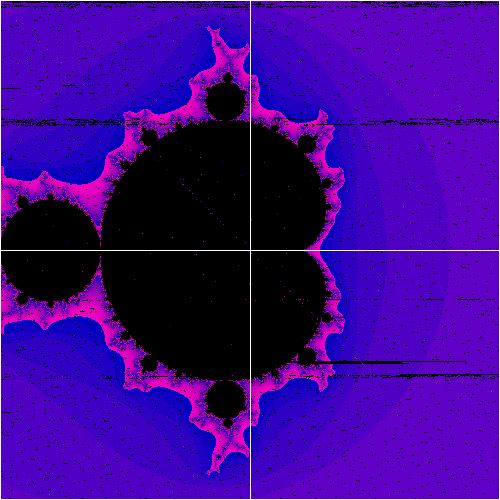
\includegraphics[width=0.5\textwidth]{einzelnVersandt.PNG}
	\caption{Mandelbrotmenge bei separatem Versand jedes einzelnen Wertes}
	\label{fig:Bild1}
\end{figure}

Um überhaupt das Bild rendern zu können, werden leere Nachrichten ignoriert und stattdessen versucht, mithilfe von vorhandenen Informationen wie dem fortlaufenden x-Wert oder dem y-Wert der berechneten Punkte, der sich bei einem Auftrag nicht mehr ändert, diese zu rekonstruieren. Der verlorene Iterationswert hingegen, kann aus diesen Daten nicht erfasst werden und soll durch den zuvor berechneten Iterationswert ersetzt werden. Da es sich dabei also nicht für jeden Punkt um den korrekt berechneten Iterationswert handelt, ist das entstehende Bild lediglich eine Approximation der Mandelbrotmenge. Dennoch entstehen eine Vielzahl an schwarzen Flecken auf der Graphik sowie falsch gesetzte Ersatzpixel. Das ist damit zu erklären, dass es nicht garantiert ist, dass auf eine verlorene Nachricht wieder eine korrekt erfasste Nachricht folgt. Somit können mehrere Nachrichten hintereinander verloren gehen, worauf dieser Ausgleichmechanismus nicht ausgelegt ist. \par

Ebenfalls erweist sich die Zeiterfassung für diese Methode der Datenübertragung als schwer. Der Client beendet seine Berechnung scheinbar wahllos und muss neu gestartet werden, um weiterhin Bildpunkte zu berechnen. Erst mit einer Konsolenausgabe, dass ein Auftrag fertig berechnet wurde, zeigt sich, dass der Client immer nach Beenden eines Auftrages anhält und keine weiteren Aufträge mehr erhält. Das lässt sich damit erklären, dass auch die Nachricht, mit der der Client neue Aufträge anfordert, vom Server als leerer String interpretiert werden kann und die Berechnung somit anhält. Lädt man den Client neu, sobald er aufhört, Punkte zu berechnen, dauert die gesamte Darstellung der Mandelbrotmenge lokal ca. 4 Minuten; ein Wert der aufgrund des wiederholten, manuellen Ladens des Clients ungenau ist.\par

Der Versuch, sämtliche berechneten Punkte durch Zeilenumbrüche getrennt in einer Nachricht zu verschicken, scheitert daran, dass die Nachricht zwar korrekt vom Server gelesen, jedoch in der Funktion, die den String übergeben bekommt, als null-String ausgegeben wird. Daher ist der nächste Schritt, diese Zeilen einzeln zu versenden. So werden x-Wert, y-Wert und die berechnete Iteration eines jeden Bildpunkts jeweils mit einem Trennzeichen aneinander gekettet und verschickt. 

\begin{figure}[htbp] 
	\centering
	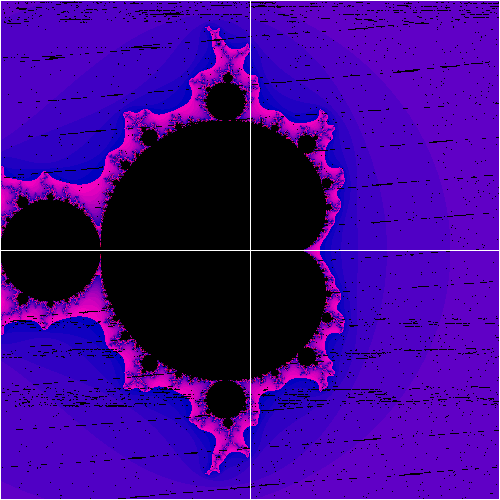
\includegraphics[width=0.5\textwidth]{zeilenVersandt.PNG}
	\caption{Mandelbrotmenge bei separatem Versand jedes einzelnen Punkts}
	\label{fig:Bild2}
\end{figure}

Da auch auf die „plot“-Nachricht vor dem Versenden der Ergebnisse verzichtet werden kann, reduziert sich die Anzahl der Nachrichten damit bei einer Bildbreite von 500 Pixeln von 2002 Nachrichten auf 502 Nachrichten.\\
Doch auch bei dieser Variante werden Nachrichten vom Server als leere Strings interpretiert und schwarze Punkte auf der Graphik gesetzt. Erneut erweist sich die Zeiterfassung als schwierig, da die Auftragsanfrage ebenfalls vom Server fehlinterpretiert werden kann, wenn auch seltener als in der zuvor verwendeten Version. Inklusive des ungenauen, manuellen Wiederverbindens des Clients, dauert die Darstellung der Mandelbrotmenge bei dieser Variante lokal ca. 70 Sekunden, was im Vergleich zu der ersten Variante einen Geschwindigkeitsgewinn darstellt. Ebenfalls lässt sich eine gewisse Regelmäßigkeit im Vergleich zu den schwarzen Punkten der ersten Variante feststellen. So scheinen die schwarzen Punkte beim zeilenweisen Versenden der Ergebnisse  diagonale Linien auf der Graphik zu ziehen. Die irregulären Anhäufungen von schwarzen Punkten geschehen hingegen immer dann, wenn der Client neugeladen werden muss. \par
Da der Server mit 502 Nachrichten pro Auftrag noch nicht in der Lage ist, sämtliche eingehende Nachrichten korrekt zu decodieren, gleichzeitig aber auch keine 500 Zeilenumbrüche in einem String verarbeiten kann, werden die Ergebnisse in der finalen Version alle in einem String pro Auftrag verschickt. Das reduziert die Anzahl der versendeten Nachrichten pro Auftrag unabhängig von der Bildbreite auf 3: eine „plot“-Nachricht, die Ergebnisse und eine Aufforderung, das Bild zu rendern. Um zu verhindern, dass keine Aufträge mehr verschickt werden und die Berechnung anhält, verschickt der Server nun selbstständig einen neuen Auftrag an den Client, sobald dieser einen abgearbeitet hat. Auf diese Weise werden keine Nachrichten mehr als leere Strings interpretiert und somit die Mandelbrotmenge vollständig angezeigt. Lokal berechnet dauert die Darstellung der Startkonfiguration in der finalen Variante bei den Maßen 500 x 500 durchschnittlich 2.4 Sekunden.\par

In der finalen Variante kann es ebenso dazu kommen, dass Nachrichten vom Server als fehlerhafte Zeichen interpretiert werden, was zu einer \enquote{NullpointerException} führt. In diesem Fall wird der Auftrag, für den die Ergebnisse erwartet werden, zurück in die Liste der Aufträge geschrieben und ein neuer Auftrag an den Client vergeben. Wenn jedoch mehrere Nachrichten und damit mehrere Reihen hintereinander vom Server als eine einzige Nachricht fehlinterpretiert werden und damit nur der erste Auftrag zurück in die Liste geschrieben wird, können vollständige Reihen in der Graphik verloren gehen. Während dieser Fehler bei der lokalen Verwendung des Clients bei den Standardmaßen selten ist, wird er bei großer Breite des Bildes häufiger und tritt bei der Verbindung zu einem nicht-lokalen Server stets auf. \par 

Die anfängliche Erwartung, dass die Integration von WebAssembly der komplizierteste Aspekt der Entwicklung des JavaScript Clients ist, erfüllt sich nicht. Diese läuft ohne Komplikationen ab und WebAssembly erweist sich als unkompliziert und verlässlich. Stattdessen ist es die Kommunikation zwischen Server und Client, die unter JavaScript deutlich mehr Probleme verursacht. Es muss nicht nur das WebSocket-Protokoll eigenhändig umgesetzt werden, sondern es treten dennoch zusätzlich einige Fehler in der Kommunikation auf, sodass Nachrichten fehlinterpretiert werden und berechnete Informationen verloren gehen. Daher empfiehlt sich eine Berechnung unter JavaScript bzw. WebAssembly nur, wenn für den Server eine Plattform gewählt wird, die das WebSocket-Protokoll unterstützt, ohne dass die Kodierung und Dekodierung einer manuellen Umsetzung bedürfen.


\section{Server}
\subsection{Funktionsweise}
Bei der ersten Version des Servers wurden jedem Client die Größe des Panels, das die Mandelbrotmenge darstellt, der Iterationswert sowie eine für jeden Client eindeutige Nummer zugewiesen. Mit diesen Kennwerten berechnete jeder Client einen gleichgroßen Bereich der Mandelbrotmenge. Dies änderte sich mit dem Wechsel zu Server Version 2.0. Fortan fragt jeder Client einen Auftrag an. Mit einem solchen Auftrag erhält der Client den y-Wert, also welche Zeile er berechnet soll, den xMove- und yMove-Wert, diese geben an wie weit sich die Mandelbrotmenge bewegt hat, den zoom-Wert, dieser gibt an wie Tief hineingezoomt wurde, und den aktuellen Iterationswert. Dies hat zur Folge, dass jetzt kein Client mehr einen bestimmten Bereich der Mandelbrotmenge berechnet, sondern nur eine Zeile pro erhaltener Nachricht. \par
Server Version 2.0 stellt die UI mittels Swing dar und die Server-Client-Kommunikation wird abhängig vom Clienttypen mithilfe von TCP bzw. des WebSocket-Protokolls realisiert, also genauso wie es bei der ersten Version war. Die Abfrage des Clienttyps wurde ebenfalls nicht verändert. \par
Wenn sich ein Client mit dem Server verbindet, dann wird mithilfe der ersten Nachricht ermittelt, um welchen Clienttypen es sich handelt und der entsprechende Thread gestartet. Nun kann ein Rechenauftrag vom Server angefordert und dieser vom Client berechnet werden. Sollte die Verbindung zum Client unterbrochen werden, bevor das Ergebnis des Auftrags an den Server geschickt wird, dann wird dieser Auftrag an das Ende der Aufgabenliste, welche alle verbleibenden Aufgaben enthält, angefügt und kann somit von einem anderem Client angefordert und berechnet werden.

\subsection{UI-Erklärung}
Bevor der Server gestartet wird, wird der User gefragt, welche Auflösung das Mandelbrotpanel haben soll. Wenn für Breite und Höhe gültige Werte (>0) eingegeben werden, startet der Server. Wenn er gestartet wird und der Port bereits belegt oder benutzt wird, dann öffnet sich ein JOptionPane und fragt den Nutzer, ob der Server neu gestartet oder ob der Vorgang beendet werden soll. Nachdem der Server erfolgreich gestartet wurde, öffnet sich die UI und die Komponenten sind zu sehen. \par
Auf der schwarzen Fläche auf der linken Seite der UI wird die berechnete Mandelbrotmenge dargestellt. Das weiße Kreuz dient dazu, die Stelle, in die hineingezoomt wird, zu zentrieren. \par
Auf der rechten Seite sind die Anzahl an verbundenen Clients sowie der aktuelle Iterationswert einsehbar. Des Weiteren wird angezeigt, wie hoch die Anzahl der Clients der verschiedenen Typen ist. \par
Am unteren Rand sind die Buttons zur Navigation zu finden. Der Restart-Button sorgt dafür, dass alle Variablen auf die Default-Werte zurückgesetzt werden und das Startbild berechnet wird. Zoom-In bzw. Zoom-Out zoomt das Bild um einen bestimmten Faktor herein- bzw. hinaus. Left, Up, Down, Right bewegen das Kreuz in die entsprechende Richtung über das Bild. Zusätzlich kann mithilfe der Tastatur herein- (Plustaste) bzw. hinausgezoomt (Minustaste) werden und mit den entsprechenden Pfeiltasten kann das Kreuz nach links, oben, unten und rechts bewegt werden. Außerdem kann mithilfe der Escapetaste die Berechnung neugestartet und mit dem Mausrad herein- bzw. hinausgezoomt werden. \par
Der Nutzer hat außerdem die Möglichkeit, mithilfe der Maus ein Rechteck über einen bestimmten Bereich zu ziehen, um in diesen hineinzuzoomen. Dabei hilft dem Nutzer ein kleines Kreuz in der Mitte des Rechtecks, um den gewünschten Bereich zu zentrieren. Um das Rechteck zu zeichnen, muss der Nutzer die linke Maustaste klicken und gedrückt halten. Wenn diese losgelassen wird, wird in das Bild hineingezoomt und neu berechnet. Falls das Rechteck an der falschen Stelle angesetzt wurde, kann die rechte Maustaste geklickt werden und der Vorgang wird abgebrochen.


\section{Reflexion}
Ziel dieses Praktikums im Großen Studienprojekt war es, ein verteiltes System zur performanten Berechnung und Visualisierung der Mandelbrotmenge zu entwickeln. Zwecks dessen wurden ein Server, der Rechenaufträge verteilt, sowie Clients, die unter Verwendung verschiedener Technologien diese Rechenaufträge annehmen und berechnen, programmiert. Während sich die Visualisierung der Mandelbrotmenge als unkompliziert erwies, ist der Faktor der Performanz deutlich hinter den Erwartungen zurück geblieben. Aufgrund der Einschränkungen durch die Pandemie konnte das verteilte System immer nur lokal getestet werden. Die Rechenleistung der Clients entsprangen demnach stets nur einem System. Ein Hosten über das Internet war nicht möglich. Ein Hosten des Servers über eine Remote-Verbindung auf einem Rechner des Universitätsnetzwerks und eine anschließende Verbindung der Clients über VPN, erzeugte einen massiven Overhead, dessen Gründe nicht bekannt sind, wodurch die Latenz zur Darstellung eines Bildes in den Minutenbereich anstieg. \par 
Auch lokal verursachte die TCP-Verbindung einen kleinen Overhead. Die Berechnungsdauer der Mandelbrotmenge im Bereich der 64 Bit double-precision ist aber niedriger als der erzeugte Overhead, sodass es im Nachhinein betrachtet nicht sinnvoll erscheint, ein verteiltes System für diese Genauigkeit zu verwenden. Falls dieses Projekt erneut angeboten werden sollte, würde es sich empfehlen, mathematische Bibliotheken zu verwenden, die eine Berechnung über die 64 Bit double-precision hinaus ermöglichen, da dort erst die rechenintensiven Berechnungen, verursacht durch hohe Iterationszahlen, entstehen. Hinzu kommen die Erkenntnisse, dass die manuelle Umsetzung des WebSocket-Protokolls zu fehlerhafter Kommunikation mit dem entsprechenden Client führen kann und das Einbinden von CUDA in ein verteiltes System nur sinnvoll ist, sobald wirklich massiver, parallelisierbarer Rechenaufwand zu bewältigen ist, da die Networkingfähigkeit von CUDA mangelhaft sind. \par 
Die Arbeit auf Distanz erwies sich als besondere Herausforderung. Da beispielsweise nicht jedes Gruppenmitglied über die benötigte Hardware verfügt, um den CUDA Client ausführen zu können, fiel ein Testen dessen schwer. Ein solches Problem hätte umgangen werden können, wäre der Zugang zu den Rechnern an der Universität möglich gewesen. Das Anlegen und Verwenden des gemeinsamen GitHub Repositorys fiel zu Beginn des Projekts noch schwer, jedoch nahmen die anfänglichen Probleme mit voranschreitender Zeit des Projekts ab, sodass sich GitHub als Versionskontrolle für das Projekt als nützlich erwies.

\nocite{*}




\end{document}

